\documentclass{article}
\usepackage{amsmath}
\usepackage{amsfonts}
\usepackage{amssymb}
\usepackage{mathrsfs}
\usepackage{cancel}

\usepackage{graphicx}


\setlength\parindent{0pt}

\author{Pranav Tikkawar}
\title{Assignment 5}

\begin{document}
\maketitle

% Strategema is the latest craze in the gaming world. In the game of Strategema, two players
% compete until a victor is determined, there can be no draws.
% Two brothers, Sven and Jens Carlsson have a friendly sibling rivalry going. To decide bragging
% rights, the two brothers play 100 games of Strategema to finally settle who is the better player.
% The attached dataset contains data from the 100 games the Carllson brothers played. The
% fields included are the game number, the winner, the loser and the time duration of the game
% (in seconds).
\section*{Question 1}
% For the games Sven won, provide an estimate of the mean time it takes Sven to beat his
% brother. Similarly, for the games Jens won, provide an estimate of the mean time it
% takes for Jens to beat his brother. –
The mean time it take Jens to beat his brother is 64.227 seconds and the mean time it takes Sven to beat his brother is 122.839 seconds.

\section*{Question 2}
% ) Construct two Q-Q plots, one displaying the durations of the games Sven won, and
% another displaying the durations of the games Jens won. (Note: When making the Q-Q
% plots, treat them as two separate datasets.) –

\begin{figure}[ht]
    \centering
    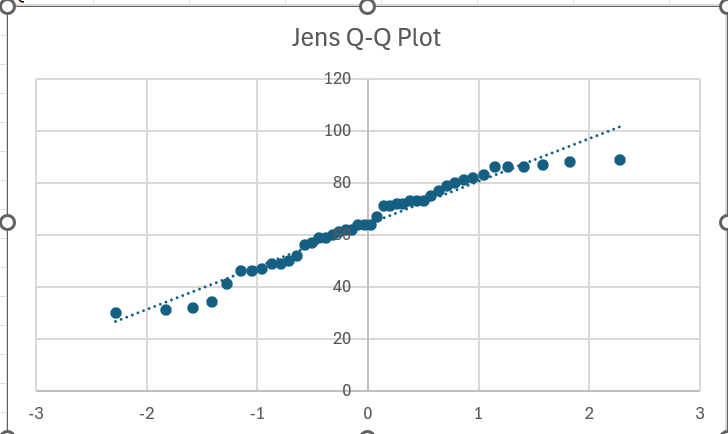
\includegraphics[width=0.5\textwidth]{A5IMG/JQQ.png}
    \caption{Q-Q plot of the durations of the games Jens won}
    \label{fig:JQQ}
\end{figure}

\begin{figure}[ht]
    \centering
    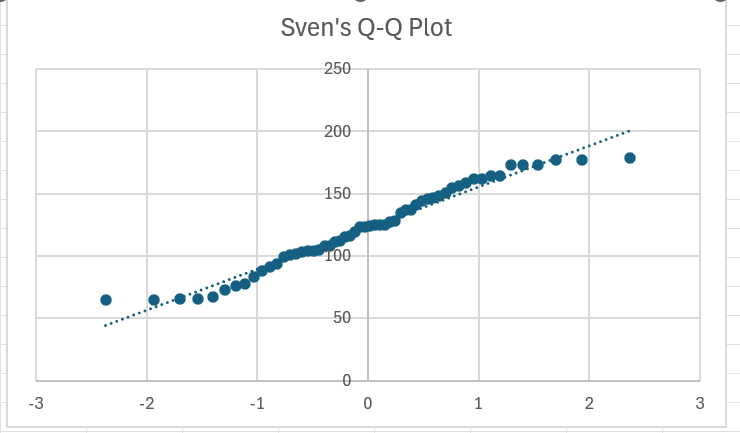
\includegraphics[width=0.5\textwidth]{A5IMG/SQQ.png}
    \caption{Q-Q plot of the durations of the games Sven won}
    \label{fig:SQQ}
\end{figure}

\section*{Question 3}
% % ) Using the QQ-Plots in part 2, is it plausible to conclude that the distribution of duration
% for the games Sven won follows a Normal Distribution? Analogously, is it plausible to
% conclude that the distribution of duration for the games Jens won follows a Normal
% Distribution? –
The distribution of duration for the games Sven won follows a normal curve near the middle of the data but tends to trail off at the ends. It looks like the example 3 in the assessing normality slides, the thin tailed distribution.\\
The distribution of duration for the games Jens won follows a normal curve near the middle of the data but tends to trail off at the ends.  It looks like the example 3 in the assessing normality slides, the thin tailed distribution.\\

\section*{Question 4}
% % Let µS denote the mean duration of games Sven wins. Similarly, let µJ denote the mean
% duration of the games Jens wins. Construct a two-sided 70% confidence interval for the
% quantity, ∆ = µS – µJ. Do not assume the standard deviation of the durations are the
% same for both brother’s wins.
The 70\% confidence interval for the difference in mean time it takes Sven to beat his brother and the mean time it takes Jens to beat his brother is $(53.25, 63.97)$

\section*{Question 5}
% Sven won 56 out of the 100 games (this can be ascertained from the dataset). Based on
% the prior fact, one might conclude Sven is the better Strategema player. After analyzing
% the game durations in the previous problems, would you agree with the assessment that
% Sven is the better player?
Despite the fact that Sven won more games, the mean time it takes Jens to beat his brother is 64.227 seconds and the mean time it takes Sven to beat his brother is 122.839 seconds. Also Jens has a lower standard deviation than Sven. So, I would say that Jens is the better player as he is more consistent and takes less time to win.


\end{document}